
Because of the resource-intensiveness of traffic simulations and the
rapid responses required by web requests, our system had to maintain a
cache of values to meet the specifications described below. We
considered two main ways of implementing this cache.

\begin{description}
    \item[Daemon] Maintain a constantly running process with the
  system code and allow the web requests to interact with this
  processes. In this scenario the cache would be program's state.
    \item[Database] Run the simulation periodically and store the
  entire output in a database and allow requests would to query this
  database. In this scenario the cache would be the database.
\end{description}

Since modularity was an important design consideration for us, we
opted for the second alternative.

\subsection{System Proposed Approach}

The system we built consists of two primary subsystems, each of which
is further divided into modules, as shown in figures
\ref{fig-back-end} and \ref{fig-front-end}.

\begin{figure}[htp]
  \centering
  \begin{subfigure}{.4\textwidth}
    \centering
    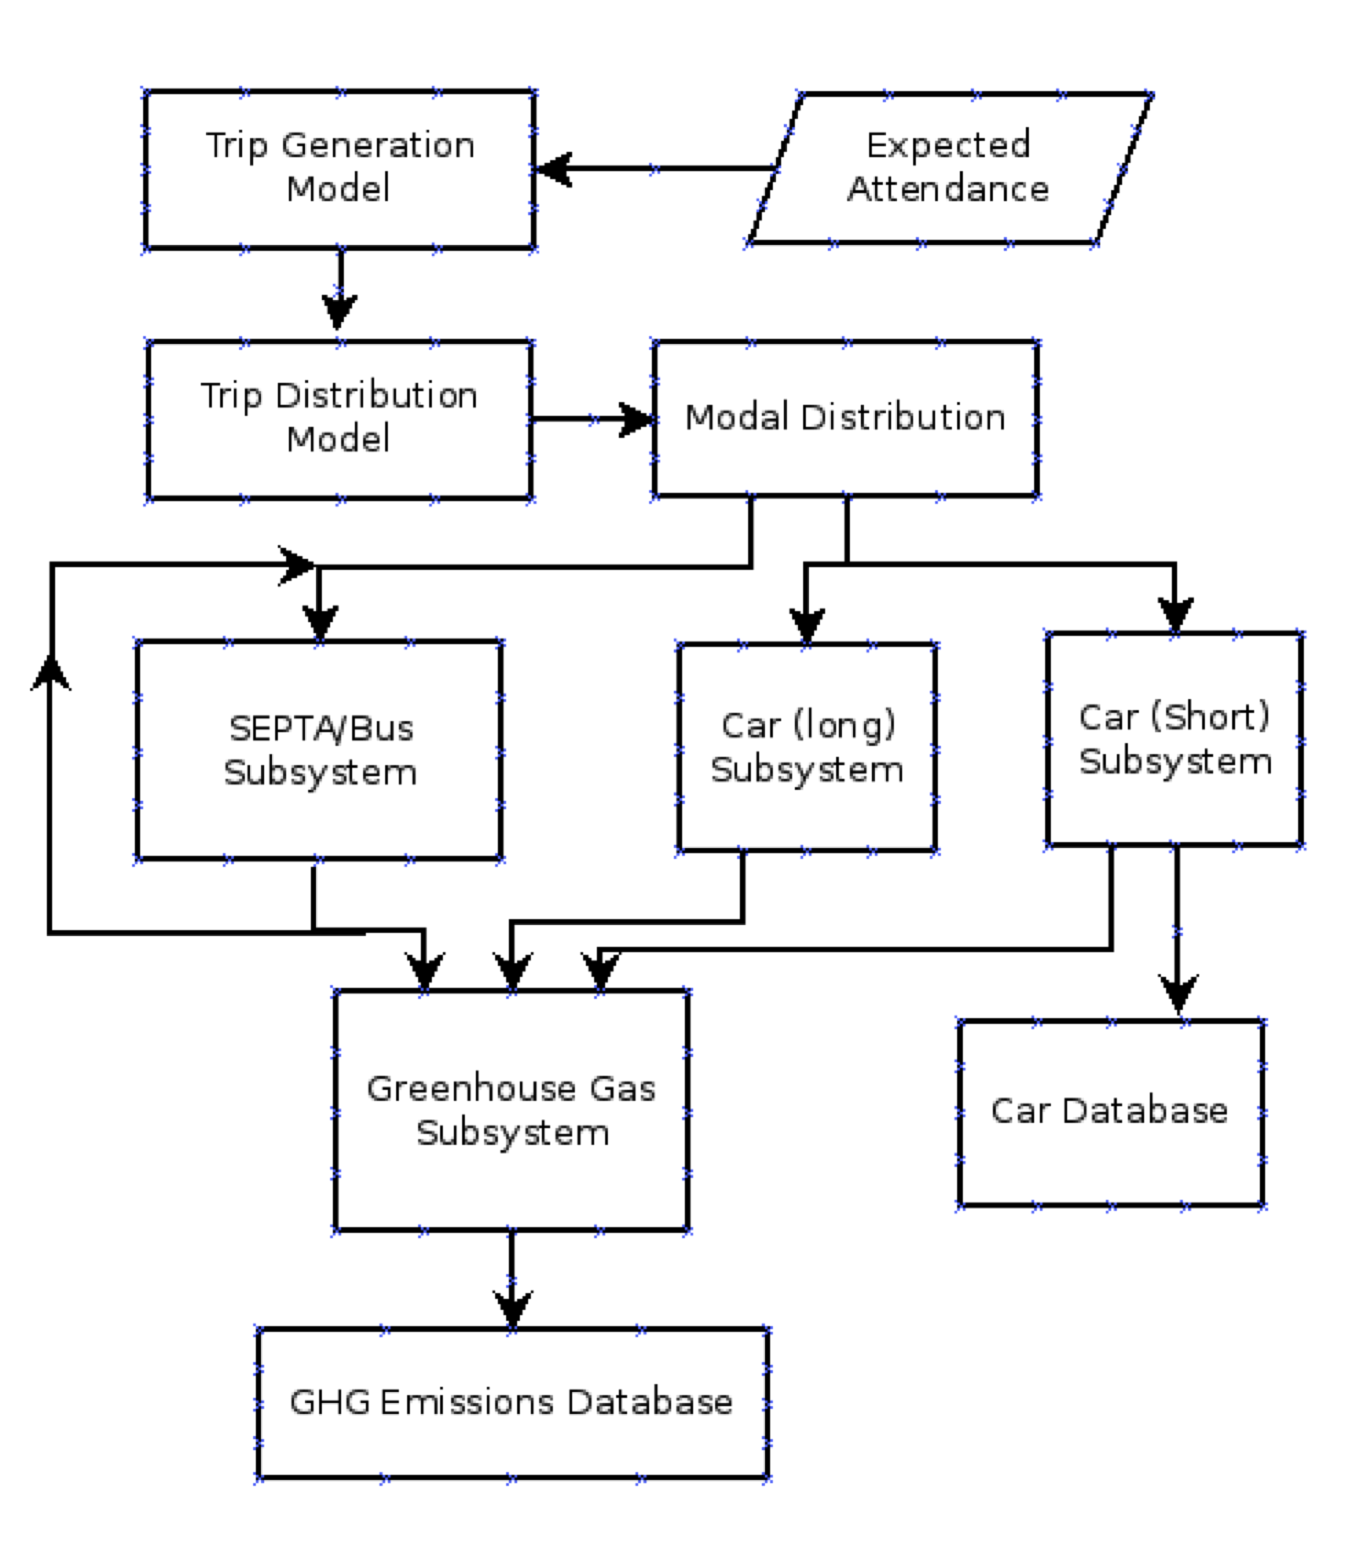
\includegraphics[height=8cm]{graphics/backend.png}
    \caption{System block diagram of our back-end model}
    \label{fig-back-end}
  \end{subfigure}
  \begin{subfigure}{.4\textwidth}
    \centering
    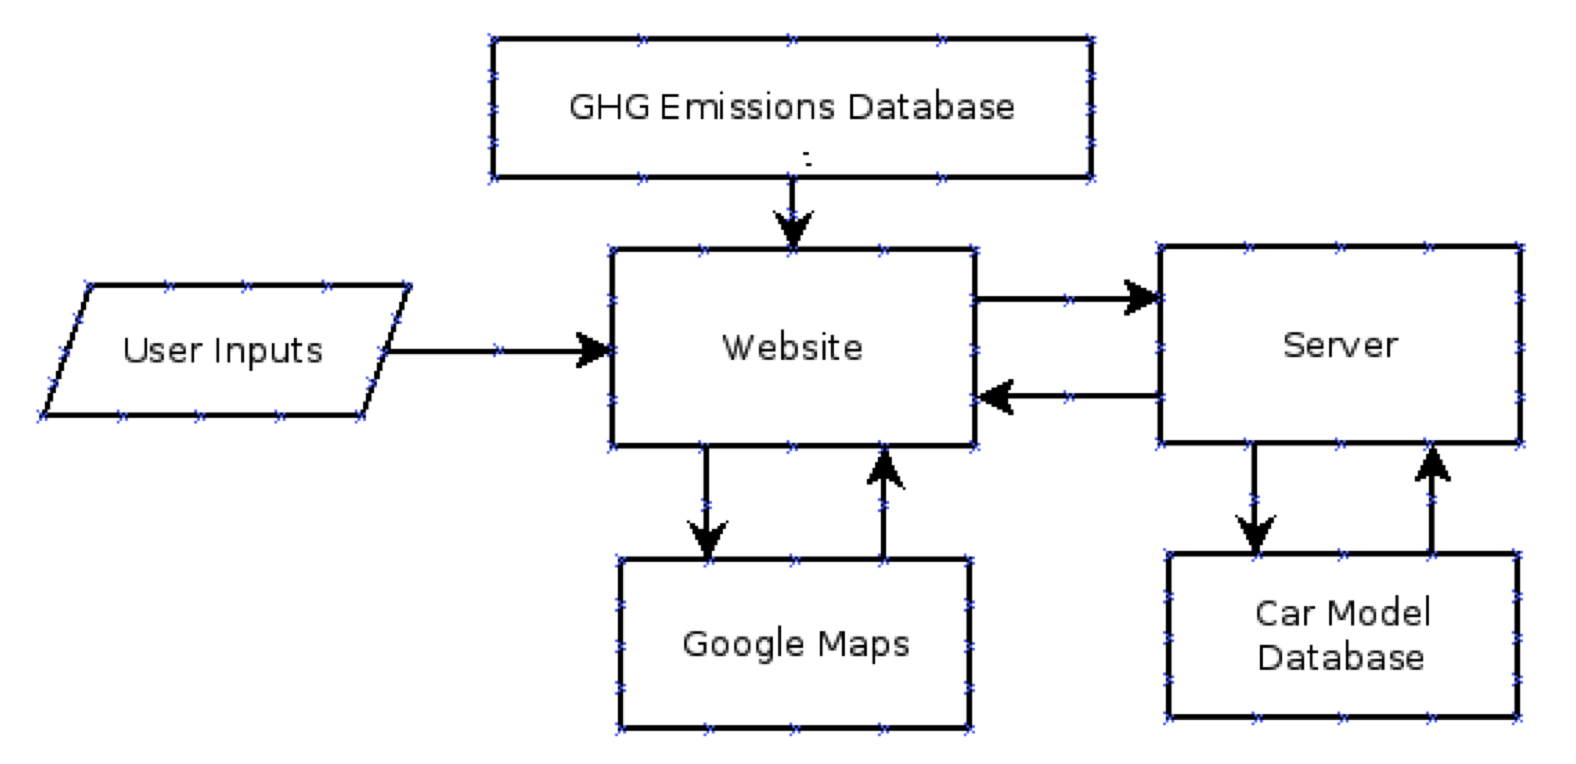
\includegraphics[height=8cm]{graphics/frontend.png}
    \caption{System block diagram of our front-end model}
    \label{fig-front-end}
  \end{subfigure}
\end{figure}

The front-end system consisted of a web server to select and display
the relevant information for a user navigating to the site. As
described in further in detail in section \ref{sec-specs}, this system
needed to be fast and lightweight. An important consideration for this
system was extensibility. Since this system depended critically on
user preferences, we wanted to be able to easily modify it as we got
feedback. Although sacrificing performance compared to some other
languages, we decided to program this part mostly in Python because
that was the language our team had the most experience
in. Furthermore, within Python we decided to implement the server
functionality as a CGI script rather than using a framework because
the script retained more of the flexibility we needed to respond to
user feedback.

The data that the website accessed was stored in a combination of
CSV files and SQLite databases. We designed the back-end of the system
to generate these files as appropriate. In keeping with the UTMS, we
structured our model around the four phases of \emph{Trip Generation},
\emph{Trip Distribution}, \emph{Modal Split}, and \emph{Trip
  Assignment}. Because of our specific intent, we also added the
\emph{Greenhouse Gas Calculator}. Each of these blocks is described in
more detail below:

\begin{description}[style=nextline]
    \item[Trip Generation] This module requires a selection of TAZs
  and estimates a geographic distribution of fans in this area. We
  decided that expected attendance would be the most reasonable input
  for this module, which then uses the Gravity Model to calculate to
  expected number of trips from each TAZ. The Gravity Model is
  described by the following equation:
  \[
    k_{i} \propto \frac{P_{i}}{r_{i}^{2}},
  \]
  where $k_{i}$ is the total number of fans in the $i$-th TAZ, $P_{i}$
  is the population of that TAZ, and $r_{i}$ is its distance from the
  stadium. The temporal distribution of the trips is then set
  according to the table in \cite{stadia-and-arenas}. This was a key
  departure from the standard transit models, since we used arrival
  times rather than departure times. We felt that this modeling choice
  more accurately reflected how people thought about the game in real
  life.
    \item[Trip Distribution] This step in the modeling was
  straightforward, since we knew that fans are traveling to and from
  the stadium or a nearby parking lot.
    \item[Mode Choice] This phase involved matching each trip in the
  database to a mode of travel (i.e. Car vs. SEPTA vs. Bus). We used
  parking-lot data to estimate car use, and corroborated it with SEPTA
  data. We left this module memoryless to retain simplicity and since
  we were focused on capturing reality for the marginal fan using the
  website, rather than modeling population-wide feedback
  phenomena. This decision also allowed us to generate some of the
  experimental results described in section \ref{sec-results}.
    \item[Trip Assignment] In traditional transit models, this phase
  corresponds to the selection of the specific lines, streets,
  highways, and stations that each trip will follow. Because of the
  unique nature of sports games (from a transit point of view), we
  broke the model into subsystems for each of the possible means
  of transportation.
    \begin{description}[style=nextline]
        \item[SEPTA] Using SEPTA's published information, we built a
      database of lines and schedules that the model used to build
      a software representation of the network. We decided to
      approximate people's behavior as though they were rational with
      perfect information and took the shortest path available to the
      stadium. To effectively deal with capacity constraints on a
      per-trip basis and generate the summary statistics that users
      wanted to see, we solved the routing problem using a
      time-expanded graph as described in \cite{george2008time} and
      \cite{schulz2000dijkstra}. We chose this method instead of the
      more traditional time-discretization approach because of the
      greater accuracy it could deliver.
        \item[Cars] Our car model was split in two: \label{cars}
      \begin{itemize}
          \item At a "micro" level, we modeled the road network in and
        around the stadium parking lot with hand-input data that we
        extracted from maps and planning documents. This portion was
        used to model the exiting cars, since we believed the
        congestion at the end of a game results in substantial GHG
        emissions, lost time, and inconvenience to the end user. This
        simulation was carried out stochastically, as described in
        \cite{van2007modeling}. We expanded the approach in that paper
        to include as many queues as we need for the parking lot
        network.
          \item At a "macro" level, we used the same TAZs as in the
        trip generation phase, and calculated a sample path to the
        stadium based on highways and main roads. We collected this
        data by hand using Google Maps.
      \end{itemize}
    \end{description}
      \item[GHG Calculator] This subsystem is a memoryless
    function mapping a trip to an estimated emissions value. Our
    preliminary assumption is that trips taken on public transit
    contribute no additional GHG, since we are taking the bus and
    train schedules as given. For cars, there are a multitude of
    published methods for estimating emissions. We will have to
    estimate a fleet profile (average age and size) to use one of
    these models. We expect that it will be a function of total
    highway distance/time, local street distance/time, and idling
    time. When properly built, the output from this subsystem will be
    our first main deliverable.
\end{description}


